
\section{The P-T Relationship of a Gas}

\makelabheader %(Space for student name, etc., defined in master.tex)

\textbf{Objectives} 

To investigate the relationship between pressure and temperature for
a constant mass of gas at constant volume and determine the value
of absolute zero.

\textbf{Apparatus} 

\begin{itemize}
\item Pasco 550 Interface
\item Pressure sensor
\item Temperature sensor
\item Air chamber and tubing
\item Hot plate
\item Glass beaker
\item Clamp and stand
\item Plastic beaker
\end{itemize}
\vspace{0.3cm}

\begin{figure}[hbt]
\begin{center}
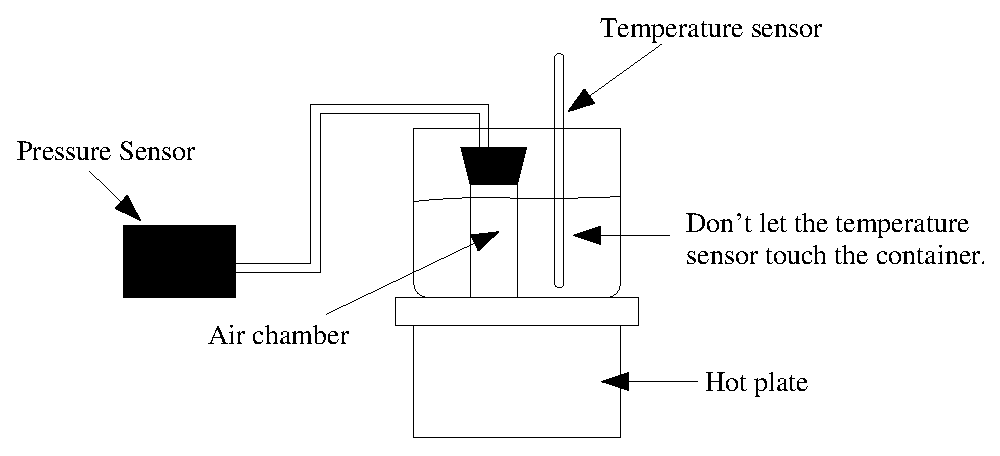
\includegraphics[width=6.0in]{P-T_relationship_of_gas/P-T_fig1b.eps}
\caption{P-T apparatus.}
\end{center}
\end{figure}

\textbf{Introduction}

The behavior of a gas can be described in terms of the macroscopic quantities:
temperature (T), pressure (P), and volume (V). The relationship between these
quantities is given by the equation of state of the gas. A real gas behaves
approximately as an ideal gas if it is far from liquefaction. In that case,
the equation of state of an ideal gas can be used to describe a real gas. For
a given mass of a gas, if one of the quantities P, T, or V is changed, a change
in the other two quantities probably will result. However, if one of the 
quantities is kept constant, the relationship between the other two can be 
studied. The relationship between temperature and pressure of an ideal gas is 
known as Gay-Lussac's law.

The experimental apparatus is shown in the figure above and consists
of an air chamber containing dry air. The volume of the gas is fixed. 
The temperature and pressure sensors are connected to the 550 Interface. 
Be sure the temperature sensor is connected to port A and the pressure sensor 
to port B. \textbf{Important:} Be sure the cables from the sensors are not touching the hot 
plate.

\textbf{Activity 1: P-T Relationship for a Gas}

%(a) Fill the beaker 3/4 full with cold tap water and place it on the hot plate.  Immerse the air chamber in the water so that most of the volume of the air chamber is submerged.  The air chamber will have to be held in place with a clamp and stand or it will float to the top.  Set the temperature sensor in the water in such a way that it is not touching the side or bottom of the beaker.

(a) The equipment should be set when you arrive in lab. The air chamber is set 
inside the glass beaker on top of the hot plate. The remparature sensor is set 
so that it is not touching the side or bottom of the beaker. Use the plastic 
beaker to fill the glass beaker about 3/4 full of cold tap water.

(b) Open the {\it P-T ss} activity in the 132 Workshop Folder under the
{\bf Start} menu.
Click on the window labeled \textit{Temperature and Pressure Table}. 
This is where your data will be displayed as you record
it. This table display will show the values of the gas pressure in the air 
chamber and the temperature of the heat bath. 
To begin recording data click
the {\bf Start} button on the {\it DataStudio} interface. 
The {\bf Start} button will change to a {\bf Keep} button and the table
display will show the values of the temperature and pressure. 
Click the {\bf Keep} button to record this temperature and pressure.

(c) Turn the hot plate on high.  As the temperature rises, click the {\bf Keep} button when the temperature is 5-7\( ^{\circ } \) above its first value.  Continue recording the temperature and pressure at 5-7\( ^{\circ } \) intervals (by clicking the {\bf Keep} button) until the water is close to boiling.  You can monitor the temperature on the temperature versus time plot to the right (on the monitor) or by watching the temperature in the \textit{Temperature and Pressure Table}.  After your last reading, click the small red box next to the {\bf Keep} button (this is the stop button) to end data recording. Turn off the hot plate.

(d) How are the pressure and temperature related?  Print your data table, enter the data in \textit{Excel} and plot pressure vs temperature on a linear graph, showing the equation of the graph.  Print this graph and add it to this unit. Write the equation here as pressure (P) as a function of temperature (T), including UNITS on the constants.
\vspace{15mm}



\textbf{Activity 2: Absolute Zero and the Kelvin Scale}

(a) The absolute zero of temperature can be defined as the temperature
at which the pressure of an ideal gas is zero. Determine absolute
zero from the equation of your graph by setting P = 0 and solving for T.
\vspace{25mm}

(b) Record the results from the other groups in the class. 
Obtain an average and standard deviation and record it here.
Are your results consistent with the class average?  Explain.
\vspace{25mm}

(c) Does there appear to be a systematic error in the class results relative 
to the accepted value of -273\( ^{\circ } \)C?  If so, what do you suppose 
causes the error? Think about this and try to explain.



